%%%%%%%%%%%%%%%%%%%%%%%%%%%%%%%%%%%%%%%%%%%%%%%% 
%%%%%%%%%%%%%%%%%%%%%%%%%%%%%%%%%%%%%%%%%%%%%%%% 
\begin{frame}
  \frametitle{Exascale race: technological challenge(s)}
  
  % https://www.exascaleproject.org/what-is-exascale/
  
  % What is Exascale?
  % Exascale refers to the next challenge in high performance computing systems: machines capable of at least a billion billion calculations per second or 50 to 100 times faster than the most powerful supercomputers in use today.  The Exascale Computing Project (ECP) was established with the goals of maximizing the benefits of high performance computing and accelerating the development of a computing ecosystem, encompassing applications, system software, hardware technologies, and architectures. An additional goal of ECP is workforce development to meet the scientific and national security mission needs of the U.S. Department of Energy (DOE) by the early- to mid-2020s.  ECP is chartered with breakthrough modeling and simulation solutions to address the most critical challenges in scientific discovery, energy assurance, and national security.  The power of this new class of systems will be measured in exaflops i.e. 1018 floating point operations per second, or a thousand times more powerful than today’s petaflop machines.
  % https://exascale.sandia.gov/
  
  \only<1>{
    \begin{minipage}{0.75\linewidth}
      \textcolor{blue}{\bf \large Exascale is about...}
      \begin{itemize}
      \item ... reaching exaflops = $10^{18}$ flop/s
        \begin{itemize}
        \item 1.3 exaflops of aggregate peak flops
        \item $\sim$ 8 PBytes of RAM
        \end{itemize}
      \item \textcolor{darkgreen}{\bf Building a computing ecosystem:} from applications, system software, hardware technologies, and architectures
      \item Doing usefull work : HPC simulation ? AI ? both !
      \item timeframe : $\sim$ 2021 - 2022
      \end{itemize}
      
      \textcolor{violet}{\bf \large Many challenges:}
      \begin{itemize}
      \item {\bf Most challenging constraint:} fitting the \textcolor{red}{\bf electrical power envelop} ( $P$ in  $[20 - 40]$ MWatts)
      \item develop new applications / adapt old ones
      \item system software, application software stacks
      \item hardware technologies ({\bf interconnect, storage, processor architectures,...})
      \end{itemize}      
    \end{minipage}
    %
    \begin{minipage}{0.24\linewidth}
      {\scriptsize {\bf Summit}\\current \#1 @top500}\\
      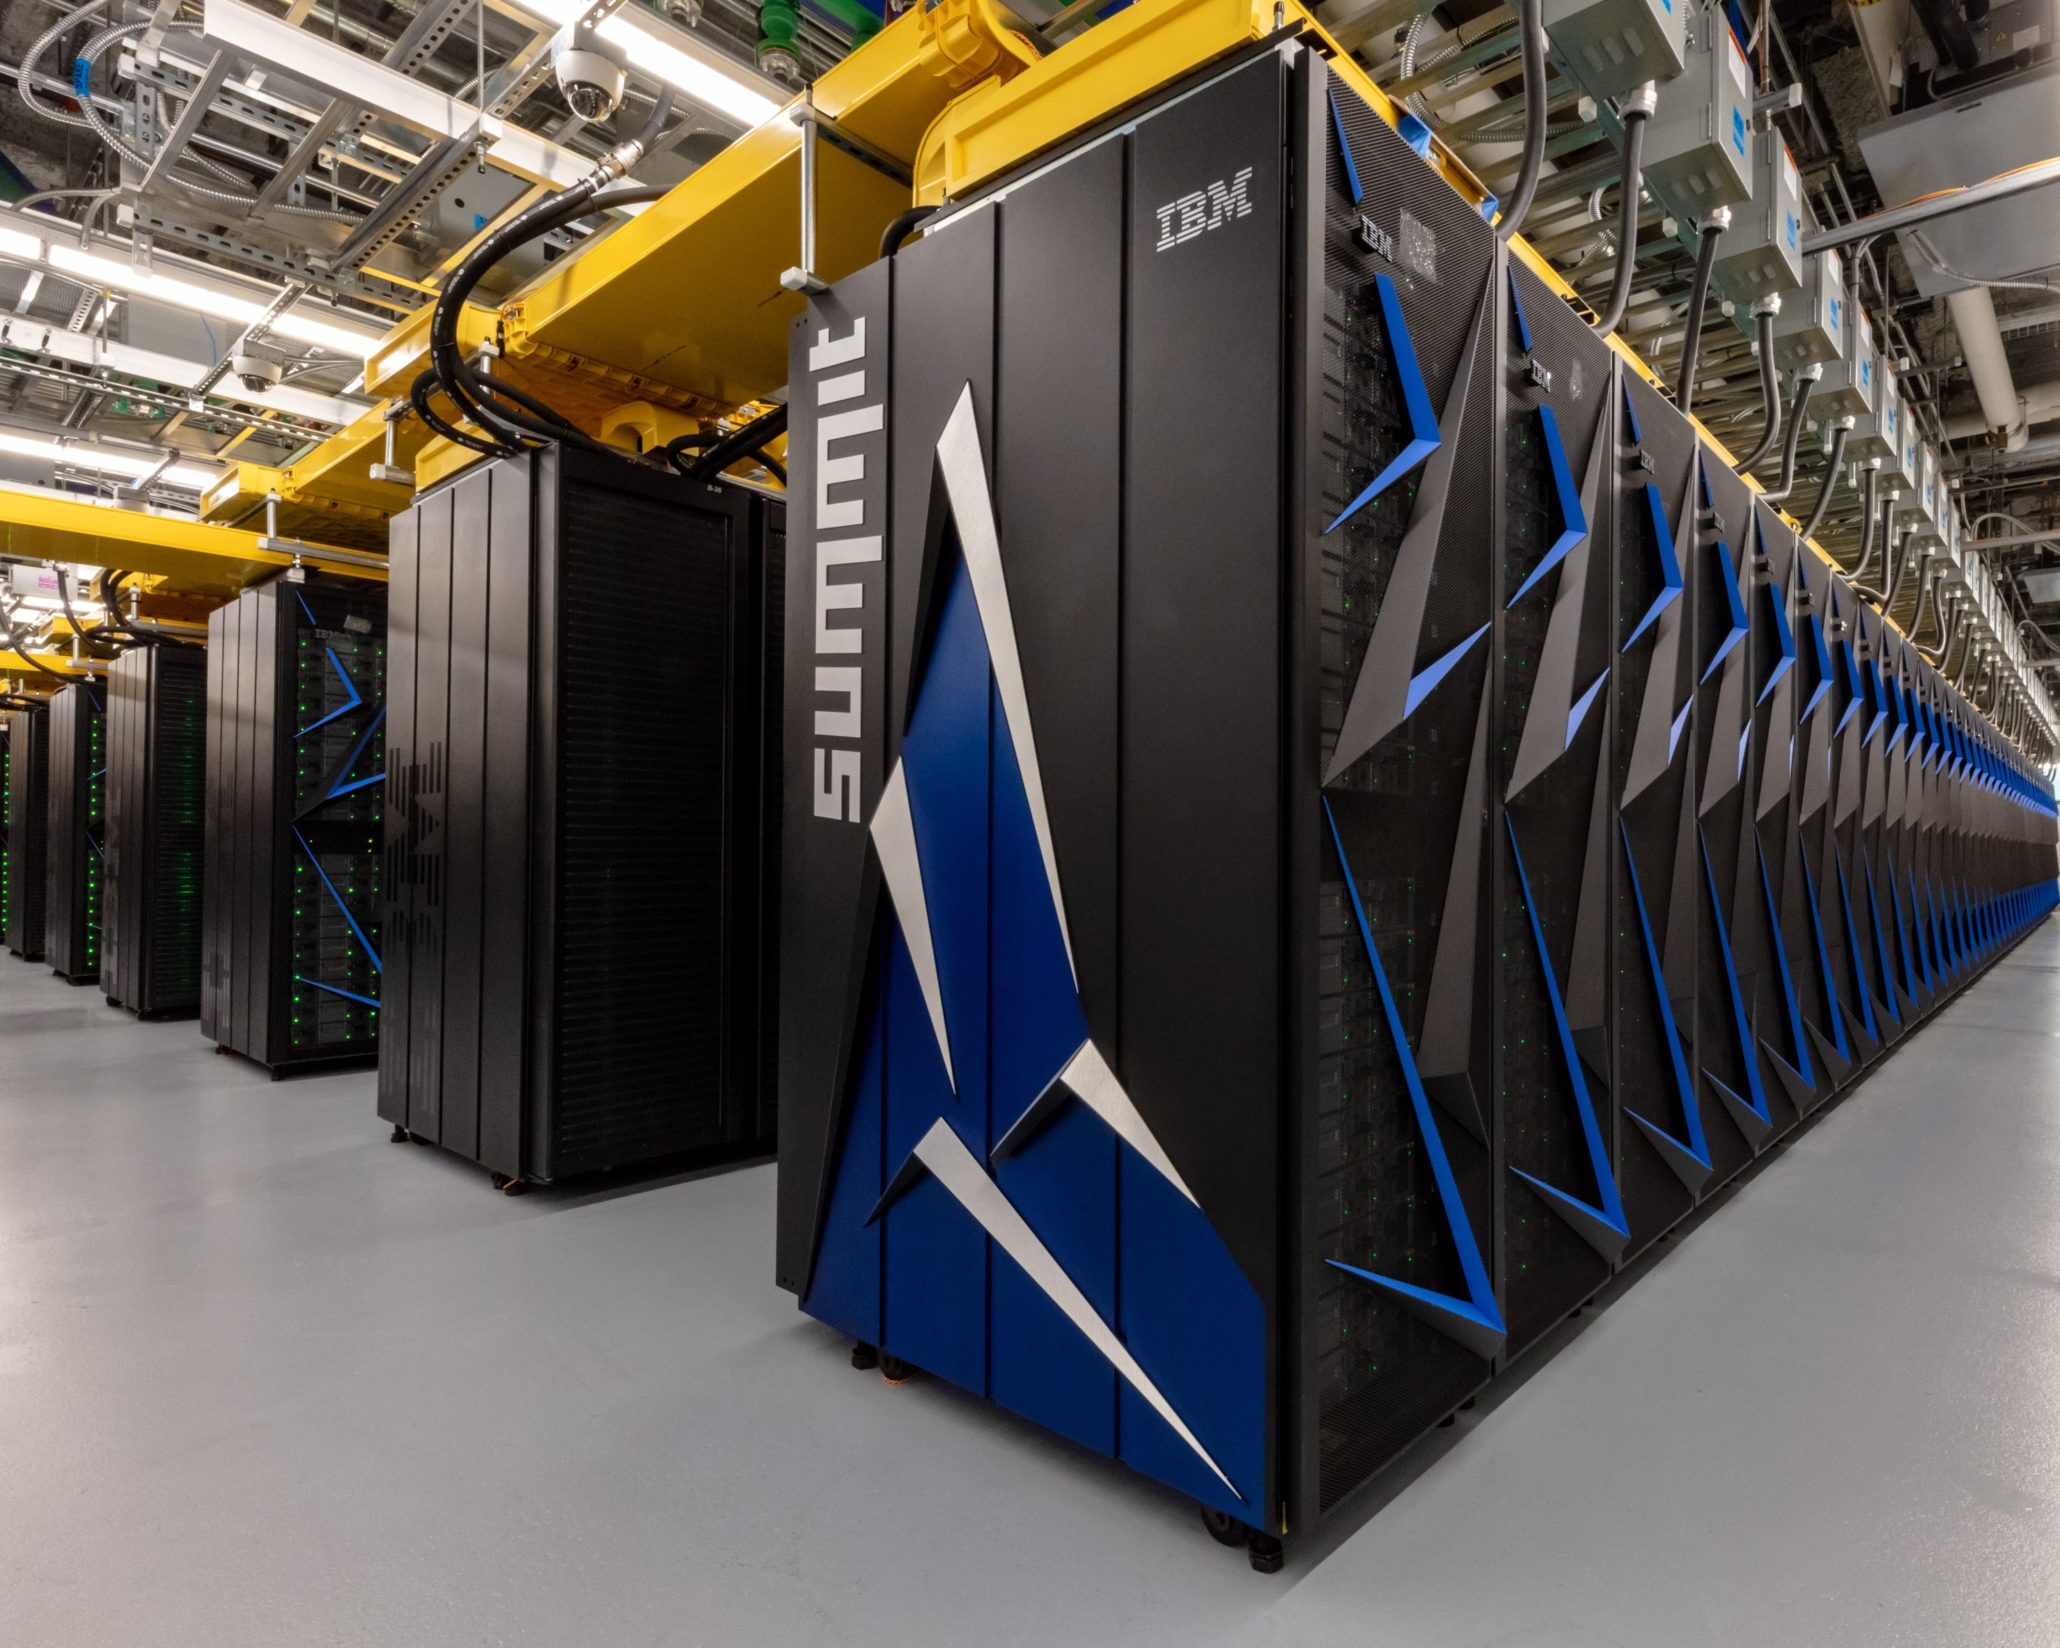
\includegraphics[width=3cm]{images/exascale/Summit_ORNL-2060x1648}
      
      {\scriptsize {\bf Post-K} (Japan, 2021 ?)}\\
      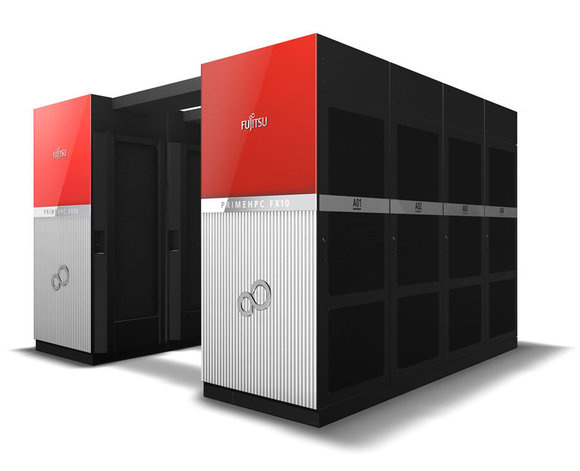
\includegraphics[width=3cm]{images/exascale/fujitsu-100677939-large}
    \end{minipage}
  }
    
  \only<2>{  
    \textcolor{violet}{\bf \large ...also about building an economic ecosystem}
    \begin{minipage}{0.68\linewidth}
      \begin{itemize}
      \item New architectures designed to address \textcolor{violet}{\bf several markets} : HPC, AI, IoT, near-sensor computing, automotive, ...
        % \item Building supercomputer is how/where real things get done
        % \item Semantic shift: HPC = ({\it old school}) simulation + ({\it more than trendy}) AI
      \item {\bf Hardware vendors already designing/optimizing new architectures for AI} (always back and forth between general purpose and application specific):e.g
        \begin{itemize}
        \item Nvidia (Tensor Core),
        \item Xilinx (Alveo / Versal),
        \item Intel (BFLOAT16, for future CooperLake), ...
        \end{itemize}
        % https://www.nextplatform.com/2018/10/02/inferring-the-future-of-the-fpga-and-then-making-it/
        % The changes in the GPU architecture to do machine learning better didn’t make GPUs any less valuable to gamers or HPC centers, but it is clear what is driving the technology.
      \item \textcolor{blue}{\bf Semantic shift: HPC = simulation + AI}
      \item \textcolor{red}{\bf Cost of designing a new chip skyrocketting, ...}
      \end{itemize}
    \end{minipage}
    % 
    \begin{minipage}{0.30\linewidth}
      \begin{center}
        {\bf Nvidia Tensor Core, Volta (2017)}\\
        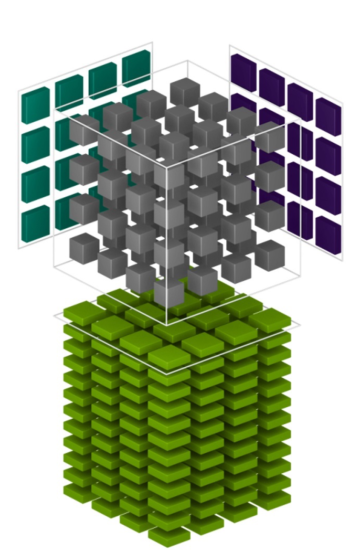
\includegraphics[width=2.2cm]{images/exascale/tensor_core_3d}
        
        {\bf Xilinx AI Engine array (2019)}\\
        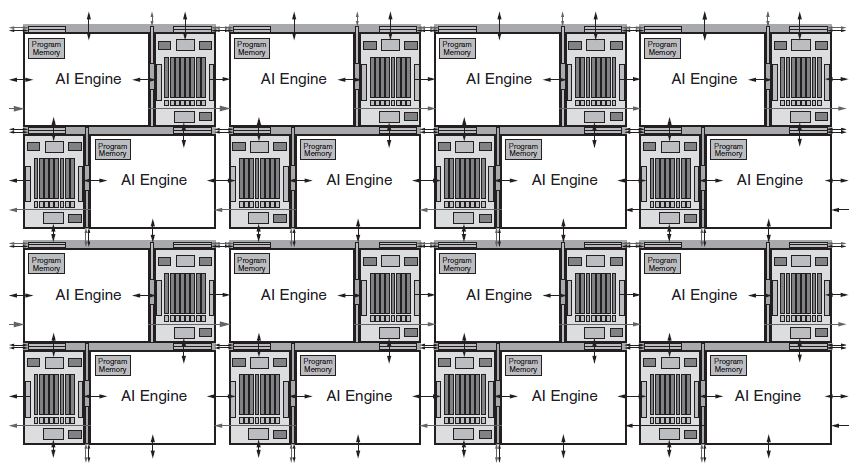
\includegraphics[width=2.5cm]{./images/exascale/Xilinx-AI-Engine-Array}
      \end{center}
    \end{minipage}
  }
  
  % https://www.nextplatform.com/2018/04/09/bidders-off-and-running-after-1-8-billion-doe-exascale-supercomputer-deals/
  
  % https://www.nextplatform.com/2018/11/12/the-widening-gyre-of-supercomputing/
  
  % from Coral to Coral-2
  % https://procurement.ornl.gov/rfp/CORAL2/
  
  % HPE the Machine :
  % https://www.nextplatform.com/2018/06/21/hpe-boots-up-sandbox-of-the-machine-for-early-users/
  % https://www.nextplatform.com/2018/06/21/hpe-boots-up-sandbox-of-the-machine-for-early-users/
  
  % can Google or Amazon Web Services or Microsoft Azure build such a machine ?
  
  % Matthieu Lobet slides : https://hal.inria.fr/hal-01820511/document
  
\end{frame}

%%%%%%%%%%%%%%%%%%%%%%%%%%%%%%%%%%%%%%%%%%%%%%%% 
%%%%%%%%%%%%%%%%%%%%%%%%%%%%%%%%%%%%%%%%%%%%%%%% 
\begin{frame}
  \frametitle{Pre-Exascale machines - hardware diversity !}
  
  \begin{itemize}
  \item \textcolor{red}{\bf \large US}: Summit , Sierra $\Rightarrow$ mostly OpenPower (IBM P9 + Nvidia V100), GPU-based architecture, \#1 and \#2 @top500
  \item \textcolor{blue}{\bf \large China:} 3 machines %(arrounds 2.5 PFlops each)
    \begin{itemize}
    \item Phytium FT2000/64 ARM chips + Matrix2000 GPDSP accelerators $\Rightarrow$ \#4 @top500, Tianhe-2A, 61 Pflops
    \item 260-core Shenwei, \textcolor{blue}{\bf homegrow technology} hardware + software (C++/fortran compiler + OpenACC) $\Rightarrow$ \#3 @top500 , Sunway TaihuLght, 93 PFlops
    \item Dhyana, AMD-licenced x86 multicore (300 M\$ !), identical to AMD EPYC
      % https://www.top500.org/news/china-reveals-third-exascale-prototype/
    \end{itemize}
    
  \item \textcolor{violet}{\bf \large Japan:} {\bf Post K}(Fujitsu, ARM, RIKEN)  A64FX ARM (\textcolor{violet}{\bf home grown}, started in 2014, 900 M\$), GPU, etc ...
    % https://www.hpcwire.com/2018/09/05/no-go-for-glofo-at-7nm-and-the-fujitsu-a64fx-post-k-cpu/
    % https://www.top500.org/news/fujitsu-reveals-details-of-processor-that-will-power-post-k-supercomputer/
    % http://www.fujitsu.com/jp/Images/20180821hotchips30.pdf
    % https://www.theregister.co.uk/2018/08/22/fujitsu_post_k_a64fx/
  \item \textcolor{darkgreen}{\bf \large Europe ?} lagging behind but new organization EuroHPC (2019), EC H2020 budget ($\sim$ 500 M\euro)\\
    \textcolor{darkgreen}{\bf home grown} ARM and/or RISC-V architecture, just starting development
    % https://www.top500.org/news/european-program-to-develop-supercomputing-chips-begins-to-take-shape/
    % mettre une EPI roadmap
    % EuroHPC (Nov. 2018 - 2026)
    % EuroHPC, Exascale not before 2022 : https://www.youtube.com/watch?v=y7_VvcIKJnI
    % EuroHPC 2 exascale machines (500 M€)
    % EuroHPC 2 pre-exascale machines in 2021 (240 M€)
  \end{itemize}

  %{\tiny \myurl{https://www.nextplatform.com/2016/07/11/chinas-triple-play-pre-exascale-systems/}}
  
\end{frame}

%%%%%%%%%%%%%%%%%%%%%%%%%%%%%%%%%%%%%%%%%%%%%%%%%%%%%%%%%%%%%%%%%%%%%%%% 
%%%%%%%%%%%%%%%%%%%%%%%%%%%%%%%%%%%%%%%%%%%%%%%%%%%%%%%%%%%%%%%%%%%%%%%% 
\begin{frame}
  \frametitle{Supercomputers architectures - TOP500}

  A Supercomputer is designed to be at bleeding edge of current technology.

  { Leading technology paths (to exascale) using \myhref{http://top500.org/lists/2013/11/}{TOP500} ranks (Nov. 2016)}
  \begin{itemize}
  \item \textcolor{blue}{\textbf{Multicore:}} Maintain complex cores, and replicate (x86, SPARC) (\#7, 10)
  \item \textcolor{blue}{\textbf{Manycore/Embedded:}} Use many simpler, low power cores from embedded (IBM BlueGene) (\#4, 9)
  \item \textcolor{darkgreen}{\textbf{Manycore/Sunway}} (\# 1)
  \item \textcolor{darkgreen}{\textbf{Manycore/Intel XeonPhi (1st and 2nd gen):}} Use many simpler cores with wide SIMD instructions, (\# 2, 5, 6)
  \item \textcolor{darkgreen}{\textbf{Massively Multithread/ GPU:}}  (\# 3, 8)
  \end{itemize}

  \textcolor{orange}{\textbf{Sunway Taihulight}} : programmed with \myhref{http://www.netlib.org/utk/people/JackDongarra/PAPERS/sunway-report-2016.pdf}{MPI+OpenACC}

  Next year, we might have supercomputers build with \textcolor{red}{\textbf{ARMv8}} CPU (From China, Japan, US,...), \textcolor{orange}{\textbf{DOE Coral machines}} (\textbf{NVidia GPU+IBM Power9, Intel KNL}), ...

\end{frame}

%%%%%%%%%%%%%%%%%%%%%%%%%%%%%%%%%%%%%%%%%%%%%%%%%%%%%%%%%%%%%%%%%%%%%%%% 
%%%%%%%%%%%%%%%%%%%%%%%%%%%%%%%%%%%%%%%%%%%%%%%%%%%%%%%%%%%%%%%%%%%%%%%% 
\begin{frame}
  \frametitle{About DOE Coral next generation computing facility}

  \begin{itemize}
  \item As part of \textcolor{orange}{\textbf{CORAL}} (Next gen supercomputers): \textbf{Center for Accelerated Application Readiness}
  \item Provide \textcolor{red}{\textbf{programming environments and tools}} that enable \textcolor{blue}{\textbf{portability}}
  \end{itemize}
  
  \begin{center}
    \includegraphics<1>[height=5.0cm]{doc/perf_portability/1-02_Straatsma_7}
    \includegraphics<2>[height=5.0cm]{doc/perf_portability/1-02_Straatsma_7_2}
  \end{center}

  {\small reference \myhref{https://www.nextplatform.com/2018/03/28/a-first-look-at-summit-supercomputer-application-performance/}{a-first-look-at-summit-supercomputer-application-performance} (March 2018)}
  
\end{frame}

%%%%%%%%%%%%%%%%%%%%%%%%%%%%%%%%%%%%%%%%%%%%%%%%%%%%%%%%%%%%%%%%%%%%%%%% 
%%%%%%%%%%%%%%%%%%%%%%%%%%%%%%%%%%%%%%%%%%%%%%%%%%%%%%%%%%%%%%%%%%%%%%%% 
\begin{frame}
  \frametitle{HPC architectures - Trends - Who's driving ?}

  \begin{minipage}{0.55\linewidth}
    \begin{itemize}
    \item \textcolor{darkblue}{\textbf{Artificial Intelligence}} applications : e.g. \textbf{Japan} (ABCI: a 130 single precision PetaFlops system in late 2017) for Companies (book time for a fee)\\
      \textbf{AI Bridging Cloud Infrastructure}: goal is 43 (FP32) GigaFlops/Watt\\
    \item \textcolor{darkgreen}{\textbf{Energy efficiency}}, e.g. \myhref{https://www.nextplatform.com/2016/11/14/nvidias-saturn-v-dgx-1-cluster-stacks/}{Nvidia's DGX-1 node} server (1 Dual Xeon + 8 GPU P100) aimed at deep learning ($\sim 18$ (FP64) GigaFlops/Watt).
    \item \textbf{Several new hardware solutions} to come next year and after: Intel Knights Mill (XeonPhi, 3rd gen), FPGA (?) for dedicated specific applications, ... \textcolor{red}{$\Rightarrow$ \textbf{a good programing model !}}
    \end{itemize}    
  \end{minipage}
  %
  \begin{minipage}{0.4\linewidth}
    \begin{center}
      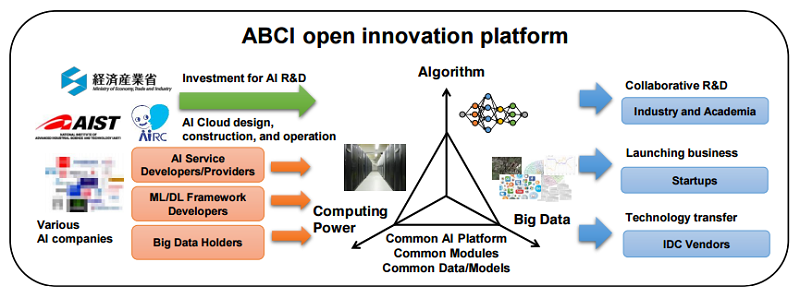
\includegraphics[width=5cm]{images/abci-innovation-800x298}
    \end{center}

    \begin{center}
      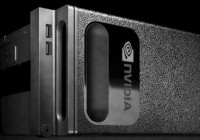
\includegraphics[width=3.5cm]{images/nvidia-dgx-1-bw-200x140}
    \end{center}
  \end{minipage}

  % \begin{itemize}
  % \item \textcolor{darkblue}{\textbf{Artificial Intelligence}} applications : e.g. \textbf{Japan} (ABCI: a 130 single precision PetaFlops system in late 2017) for Companies (book time for a fee)\\
  %   \textbf{AI Bridging Cloud Infrastructure}: goal is 43 (FP32) GigaFlops/Watt\\
  % \item \textcolor{darkgreen}{\textbf{Energy efficiency}}, e.g. \myhref{https://www.nextplatform.com/2016/11/14/nvidias-saturn-v-dgx-1-cluster-stacks/}{Nvidia's DGX-1 node} server (1 Dual Xeon + 8 GPU P100) aimed at deep learning ($\sim 18$ (FP64) GigaFlops/Watt).
  % \item Many new hardware solutions to come next year and after: Intel Knights Mill (XeonPhi, 3rd gen)
  % \end{itemize}

\end{frame}

%%%%%%%%%%%%%%%%%%%%%%%%%%%%%%%%%%%%%%%%%%%%%%%%%%%%%%%%%%%%%%%%%%%%%%%% 
%%%%%%%%%%%%%%%%%%%%%%%%%%%%%%%%%%%%%%%%%%%%%%%%%%%%%%%%%%%%%%%%%%%%%%%% 
\begin{frame}
  \frametitle{Supercomputer node architecture}

  \begin{center}
    \textbf{Multiples levels of hierarchy:}
    \begin{itemize}
    \item Need to aggregate the computing power of several 10 000 nodes !
    \item network efficiency: latency, bandwidth, topology
    \item memory: on-chip (cache), out-of-chip (DRAM), IO (disk)
    \item emmerging \textbf{hybrid programming model: MPI + X}
    \item \textcolor{red}{What is \textbf{X} ? OpenMP, OpenAcc, ..., \myhref{https://github.com/kokkos/kokkos}{Kokkos}, \myhref{https://github.com/llnl/raja}{RAJA}, ...}
    \item \textcolor{blue}{Even at node level MPI+X is required:} e.g. KNL
    \end{itemize}
  \end{center}

  \begin{figure}
    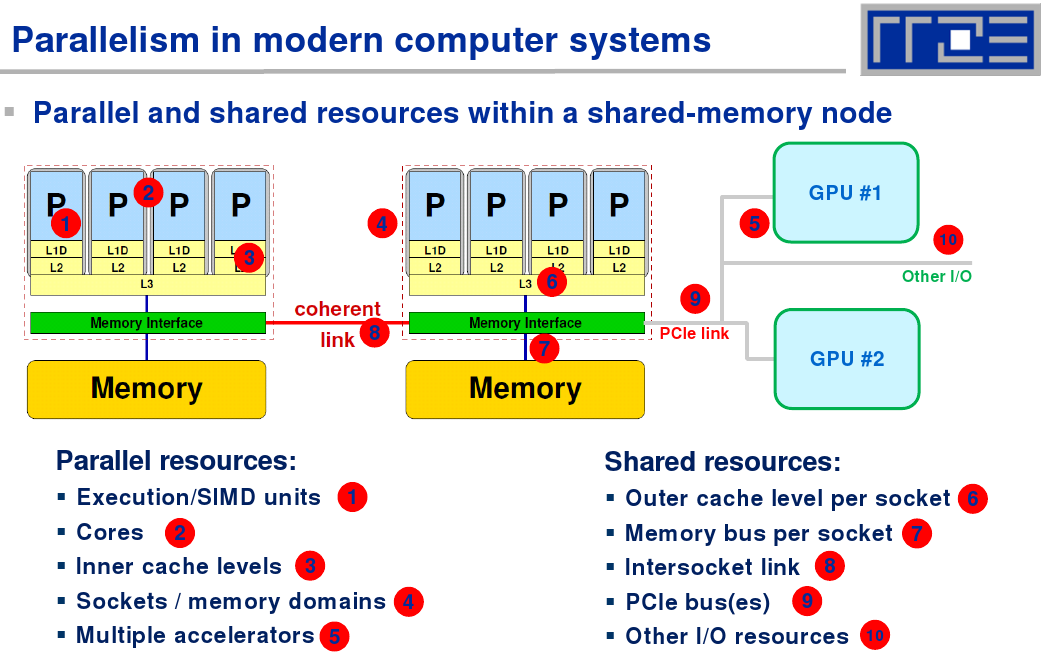
\includegraphics[width=5cm]{images/multicore_hardware}
    \caption{\scriptsize{Multi-core node summary,
        source: multicore tutorial (SC12) by G. Hager and G. Wellein}}
  \end{figure}
  
\end{frame}

%%%%%%%%%%%%%%%%%%%%%%%%%%%%%%%%%%%%%%%%%%%%%%%%%%%%%%%%%%%%%%%%%%%%%%%% 
%%%%%%%%%%%%%%%%%%%%%%%%%%%%%%%%%%%%%%%%%%%%%%%%%%%%%%%%%%%%%%%%%%%%%%%% 
% \begin{frame}
%   \frametitle{More heterogeneous  future...}

%   \begin{figure}
%     \includegraphics[height=6.5cm]{images/kokkos_heterogeneous}
%     \caption{
%       source: kokkos tutorial (GTC2014) by Carter Edwards}
%   \end{figure}
  
% \end{frame}


%%%%%%%%%%%%%%%%%%%%%%%%%%%%%%%%%%%%%%%%%%%%%%%%%%%%%%%%%%%%%%%%%%%%%%%% 
%%%%%%%%%%%%%%%%%%%%%%%%%%%%%%%%%%%%%%%%%%%%%%%%%%%%%%%%%%%%%%%%%%%%%%%% 
% \begin{frame}
%   \frametitle{What is a supercomputer ?}
  
%   % Power Efficiency over time
%   \begin{figure}
%     \includegraphics[height=6cm]{images/power_efficiency_horst_simon}
%     \caption{\myhref{http://www.extremetech.com/computing/155941-supercomputing-director-bets-2000-that-we-wont-have-exascale-computing-by-2020}{Horst Simon, LBNL}}
%   \end{figure}
  
% \end{frame}
